\begin{table}
    {\renewcommand{\arraystretch}{1.3}%
    \setlength{\tabcolsep}{0.3em}%
    \begin{tabular}{ccccccc}
    \toprule
    \null &
        \textbf{Synthetic$_{\mathbf{\mathcal{F}}}$} &
        \textbf{Lehrpfad$_{\mathbf{\mathcal{F}}}$} &
        \textbf{Office$_{\mathbf{\mathcal{F}}}$} &
        \textbf{Synthetic$_{\mathbf{\mathcal{\beta}}}$} &
        \textbf{Lehrpfad$_{\mathbf{\mathcal{\beta}}}$} &
        \textbf{Office$_{\mathbf{\mathcal{\beta}}}$} \\
    \midrule
    \rowcolor{lightgray}
    \textbf{Keypoint Count} &
        \num{15861} & \num{321526} & \num{30616} &
        \num{7810} & \num{243226} & \num{21093} \\
    \textbf{Correspondences} &
        \num{6158} & \num{23030} & \num{5289} &
        \num{3604} & \num{11405} & \num{2443} \\
    \rowcolor{lightgray}
    \textbf{True Positives} &
        \num{5994} & \num{18483} & \num{4525} &
        \num{3554} & \num{8353} & \num{2124} \\
    \textbf{False Positives} &
        \num{4010} & \num{108457} & \num{9349} &
        \num{1730} & \num{85116} & \num{7085} \\
    \rowcolor{lightgray}
    \textbf{Precision} &
        \num{0.599} & \num{0.146} & \num{0.326} &
        \num{0.673} & \num{0.089} & \num{0.231} \\
    \textbf{Recall} &
        \num{0.973} & \num{0.803} & \num{0.856} &
        \num{0.986} & \num{0.732} & \num{0.869} \\
    \rowcolor{lightgray}
    \textbf{Accuracy} &
        \num{0.736} & \num{0.648} & \num{0.665} &
        \num{0.771} & \num{0.637} & \num{0.644} \\
    \textbf{Youden-Index} &
        \num{0.557} & \num{0.439} & \num{0.480} &
        \num{0.572} & \num{0.364} & \num{0.483} \\
    \bottomrule
    \end{tabular}
    }
    \caption{Performance indicators for the default configuration of the SIFT algorithm on the different datasets.}
\end{table}
Raw numbers and absolute numbers for the recognition performance of SIFT features.
The ratios and relative performance numbers are similar between both conversions.
In absolute numbers, the \glspl{flexion-image} result in more detected features.
This higher number results in potentially better RANSAC results, because there are more correspondences to pick from.
\begin{figure}[H]
\begin{subfigure}[t]{0.45\linewidth}
    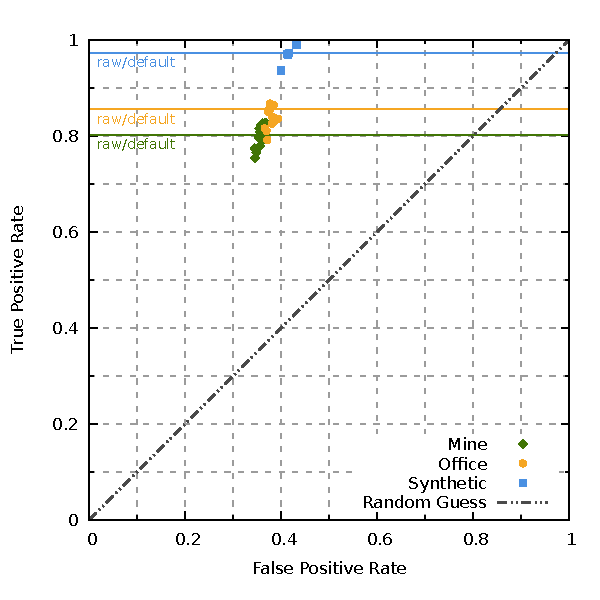
\includegraphics[width=\linewidth]{chapter06/results/SIFT/flexion/roc.pdf}%
    \caption{Flexion Image ROC}
\end{subfigure}\quad
\begin{subfigure}[t]{0.45\linewidth}
    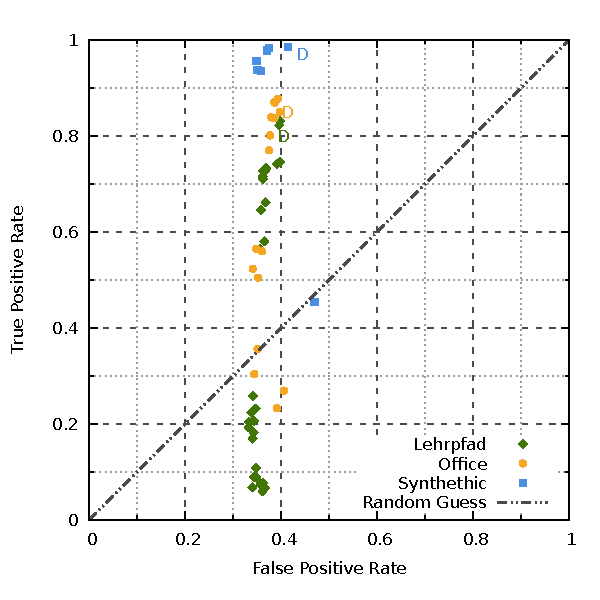
\includegraphics[width=\linewidth]{chapter06/results/SIFT/bearing/roc.pdf}
    \caption{Bearing-Angle Image ROC}
\end{subfigure}
    \caption{The ROC plot for SIFT shows a high variability for the true positive rate, but an almost constant false positive rate regardless of conversion image type.}
\end{figure}
The overall performance differences are shown here.
False positive rate does not change significantly with different algorithm parameters.
True positive rate has a wide variety.
\begin{figure}[H]
    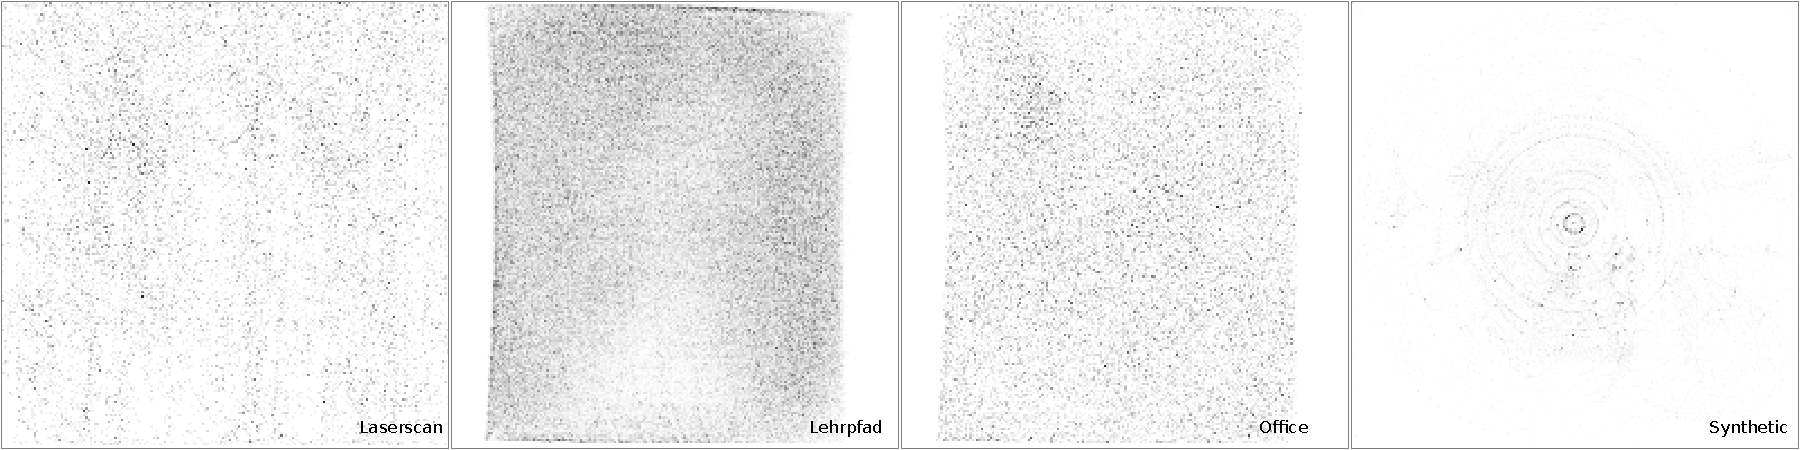
\includegraphics[width=\linewidth]{chapter06/results/SIFT/flexion/distribution.pdf}\\
    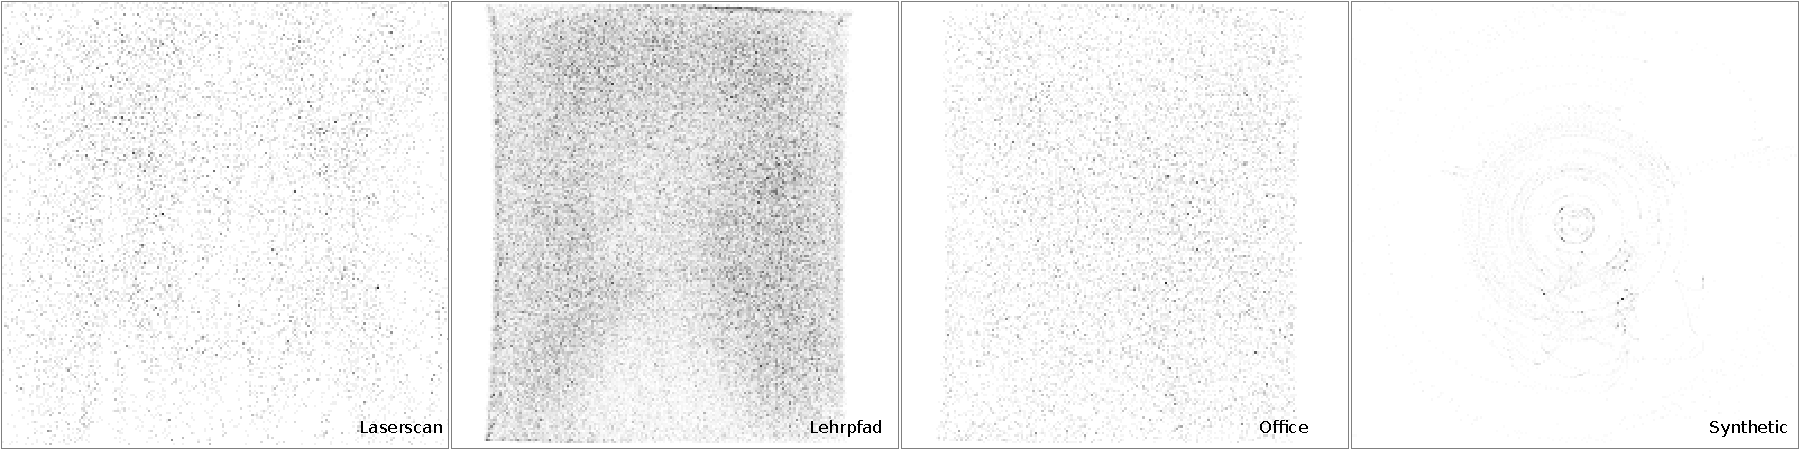
\includegraphics[width=\linewidth]{chapter06/results/SIFT/bearing/distribution.pdf}%
    \caption{The keypoint distribution for the different datasets show both good spread and that the information in the image is clearly tracked in the Synthetic dataset. The first row is the \gls{flexion-image} and the second row the \gls{bearing-angle-image} conversion.}
\end{figure}
The keypoints stick to salient regions and are not randomly distributed, as can be seen in the Synthetic dataset.
For the bigger datasets with real world geometry the keypoints are distributed all over the images, indicating not clear disfunctionality in the detection.
Flexion images create more keypoints.
\begin{figure}[H]
\begin{subfigure}[t]{0.45\linewidth}
    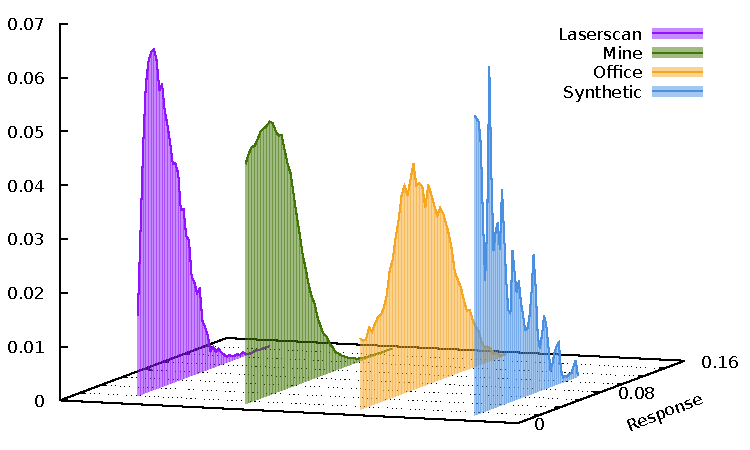
\includegraphics[width=\linewidth]{chapter06/results/SIFT/flexion/response.pdf}%
    \caption{\gls{flexion-image} Keypoint Responses}
\end{subfigure}\quad
\begin{subfigure}[t]{0.45\linewidth}
    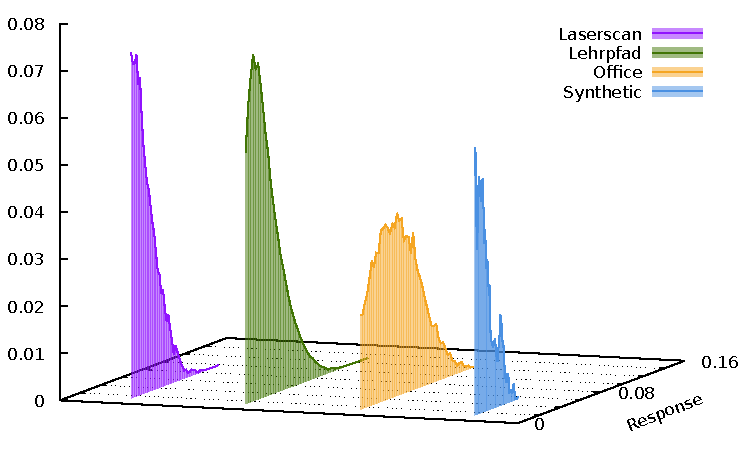
\includegraphics[width=\linewidth]{chapter06/results/SIFT/bearing/response.pdf}%
    \caption{\gls{bearing-angle-image} Keypoint Responses}
\end{subfigure}
\end{figure}
The responses show the difference between flexion images and bearing angle images.
Flexion images have a wider range of responses and on average an higher response to the keypoint detector.
The underlying distribution is similar, but bearing performs worse.
\begin{figure}[H]
\begin{subfigure}[t]{0.45\linewidth}
    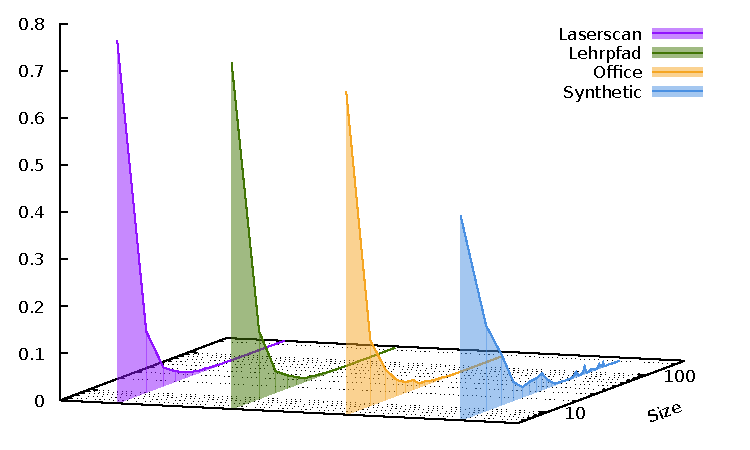
\includegraphics[width=\linewidth]{chapter06/results/SIFT/flexion/size.pdf}%
    \caption{\gls{flexion-image} Keypoint Sizes with logarithmic scale}
\end{subfigure}\quad
\begin{subfigure}[t]{0.45\linewidth}
    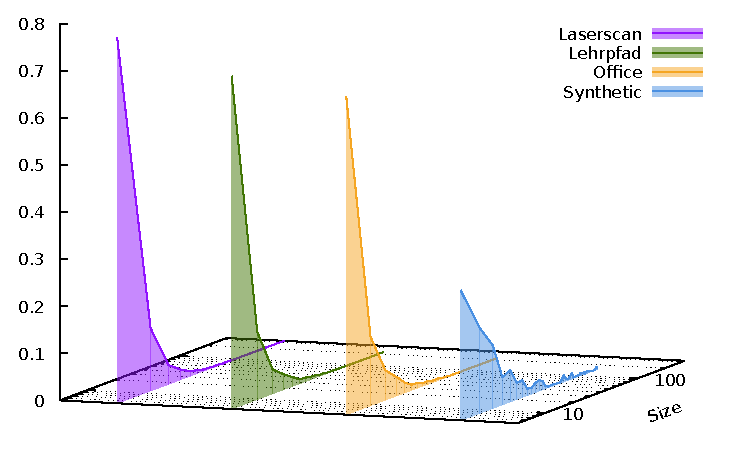
\includegraphics[width=\linewidth]{chapter06/results/SIFT/bearing/size.pdf}%
    \caption{\gls{bearing-angle-image} Keypoint Sizes with logarithmic scale}
\end{subfigure}
\end{figure}
Both conversion types have a very high skew towards small features.

\begin{figure}[H]
\begin{subfigure}[t]{0.45\linewidth}
    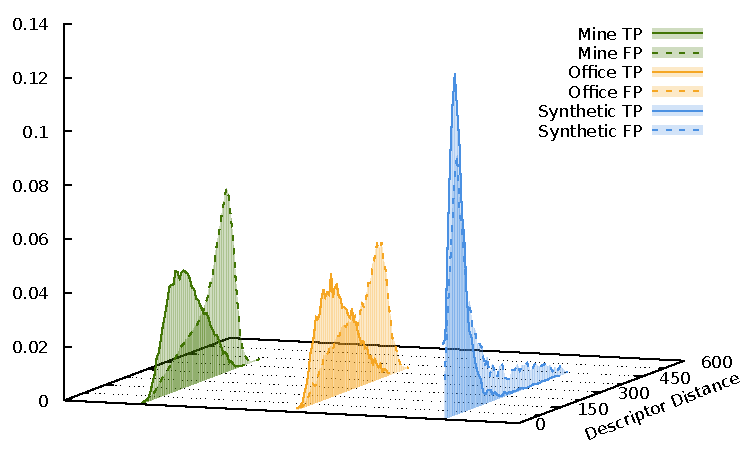
\includegraphics[width=\linewidth]{chapter06/results/SIFT/flexion/descriptor_distances.pdf}%
    \caption{\gls{flexion-image} Descriptor Distances}
\end{subfigure}\quad
\begin{subfigure}[t]{0.45\linewidth}
    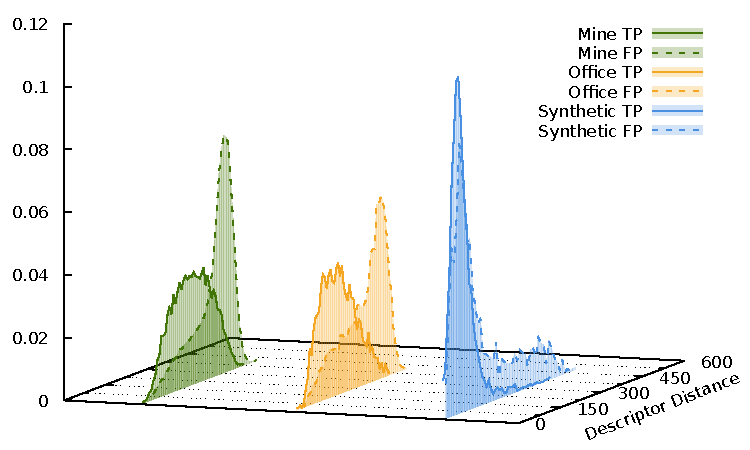
\includegraphics[width=\linewidth]{chapter06/results/SIFT/bearing/descriptor_distances.pdf}%
    \caption{\gls{bearing-angle-image} Descriptors Distances}
\end{subfigure}
\end{figure}
The analyzing the descriptor distances for true positives and false positives show skewed distributions that indicate a partial separapibility for the real world datasets.

On all datasets the only factor improving the result further was applying a threshold on the keypoint response.
Either by taking only the best $N$ points or enforcing a lower bound on the response.
This change improved the true positive rate by $~0.03$, which is only a slight improvement.

